\documentclass[12pt]{article}

\usepackage[english]{babel}
\usepackage[utf8]{inputenc}
\usepackage{amsmath}
\usepackage{graphicx}


\graphicspath{ {images/} }

\title{CS 5876 - HW 2}

\author{Joshua Campbell (jac677) , Michael Wang (mzw4) , Neil Parker (nwp7) }

\date{\today}

\begin{document}
\maketitle

\begin{enumerate}

\item[1.1)]
The idea of k-means is to minimize the sum of squared distances of each point to its cluster center (the centroid) according to the `Foundations of Data Science' by John Hopcroft and Ravindran Kannan. We try to exploit this in our solution\\
To generate our dataset, we equally spaced 30 points on a circle, split the circle in half, and then translated one of the halves. As you can see in the picture below, the halves are now intersecting. By placing the the centroids in the center of each half circle, we created a fragile situation that enabled the means to change drastically. This situation was made worse because the the half circles are intersecting; the centroids will approximately mirror each other when they are recalculated each iteration. Because of this symmetric mirroring effect, the centroids each capture 15 points in their clusters. The centroids were especially easy to change since there were not two "natural clusters" in our the dataset.

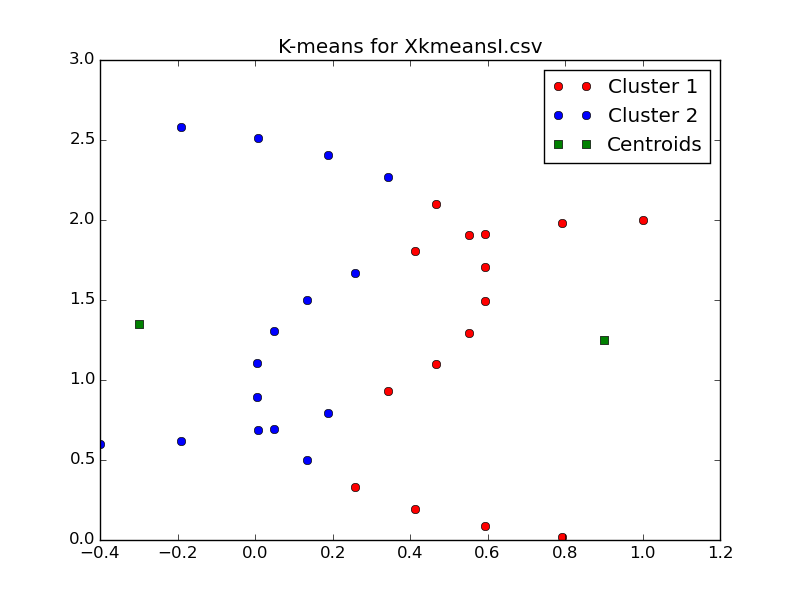
\includegraphics[width=0.5\textwidth]{K-means_for_XkmeansI.png}

To make the clusters change drastically, all we had to do was disturb the balance. We added two points close together (now classified as red) and one point near the bottom (classified as blue). This would have shifted the centroid on the left upwards, out of sync with the cluster on the right, allowing it to capture more of the right cluster's top points. Eventually, the centroid rotated about 90 degrees from their starting position.

The vary amount between clusterings was 0.4.

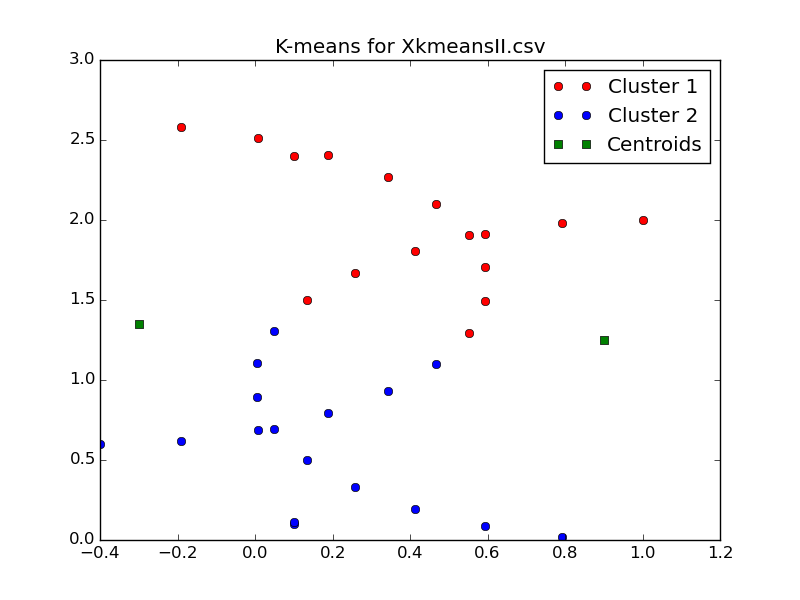
\includegraphics[width=0.5\textwidth]{K-means_for_XkmeansII.png}

\item[1.2)] The weakness with single link is that always connects the closest two points that are in different clusters. This makes it easy to manipulate. We created this dataset by creating two clusters that were separated by a gap larger than the distances between points within the clusters. This assured that single link clustering would separate the two clusters. Further more, we made the gaps between the points within a cluster successively bigger as they got further from the space between the clusters. This ensured that if the two clusters were somehow connected, all the points save one would be deterministically classified into a single cluster, allowing for the variance criteria. we put the same number of points in each cluster, obviously, to meet the criteria.

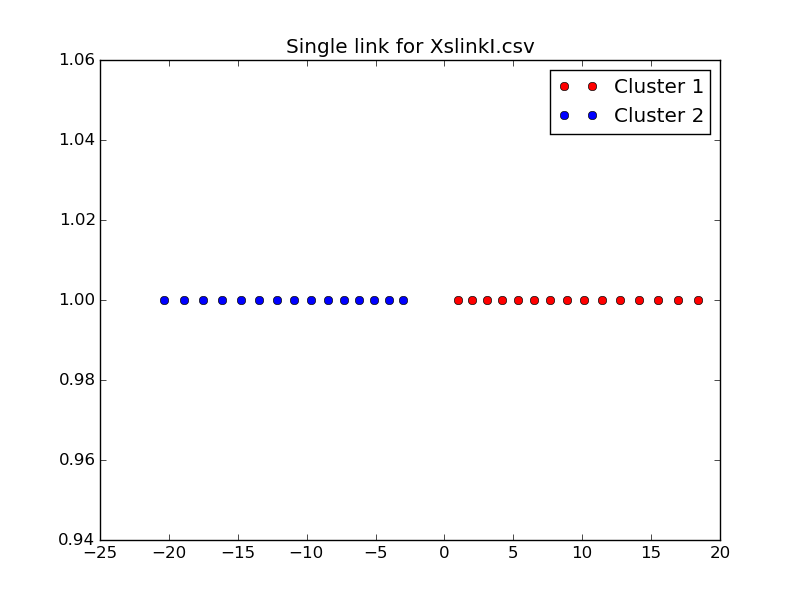
\includegraphics[width=0.5\textwidth]{Single_link_for_XslinkI.png}

To modify the clusters, we simply put three points in the gap between the clusters. The distance between these points and the between the corresponding clusters are smaller than the distances previously constructed. This ensured that the new points would be connected in one cluster and then successively be connected to points in the two original clusters.

The vary amount between clusterings was 0.4666 (repeating).

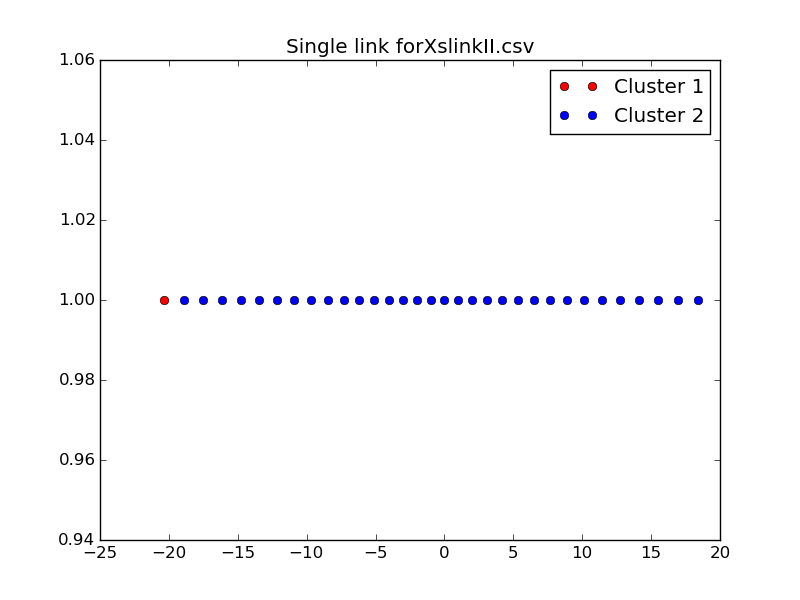
\includegraphics[width=0.5\textwidth]{Single_link_forXslinkII.png}

\item[1.3)] To construct the original graph we created two disconnected components. Because of the disconnect, they should naturally be clustered by spectral decomposition as two separate clusters. Since we used k-means on the embedding, we just had to position the centroid appropriately to capture these two clusters, as shown. 

Below is the k-means embedding, followed by the actual graph.

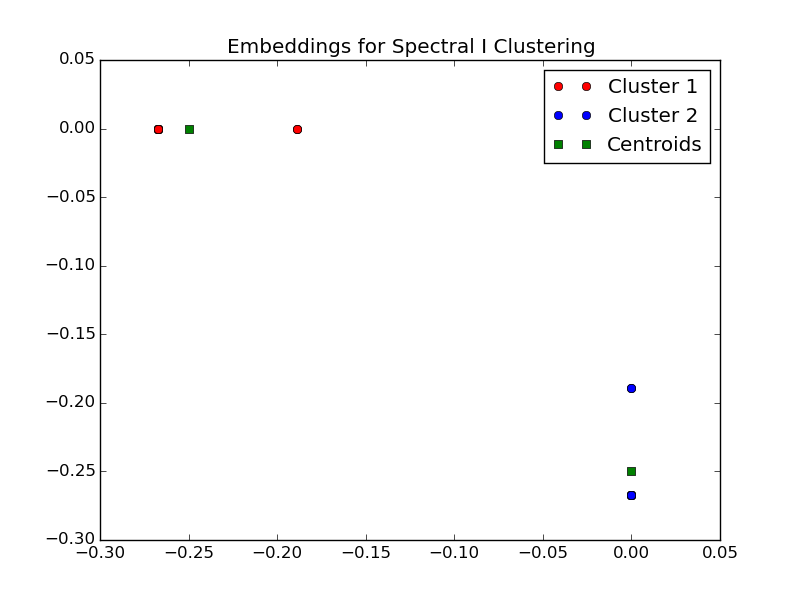
\includegraphics[width=0.5\textwidth]{Embeddings_for_Spectral_I_Clustering.png}

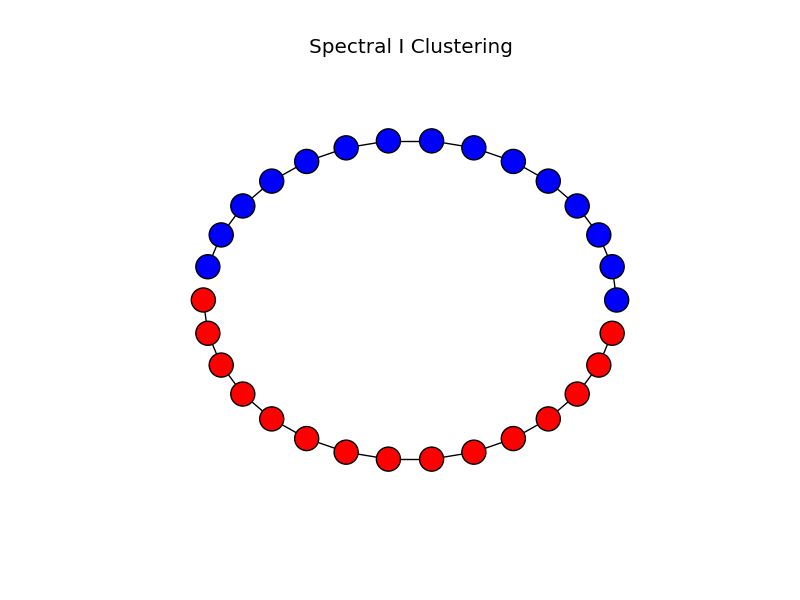
\includegraphics[width=0.5\textwidth]{Spectral_I_Clustering.png}

We added three edges in total, two to connect the original clusters so that the graph now formed a ring, and one to bridge the midpoints of the original clusters. The justification for this was that spectral decomposition would result in either the edges to the left or right of the midpoints being broken, separating the points into two separate clusters. Either way, we was sure that the k-means embedding would be vastly different since the previous graph had two components, while the modified graph only had a single component.

Below is the k-means embedding, followed by the actual graph.

The vary amount between clusterings was 0.5.

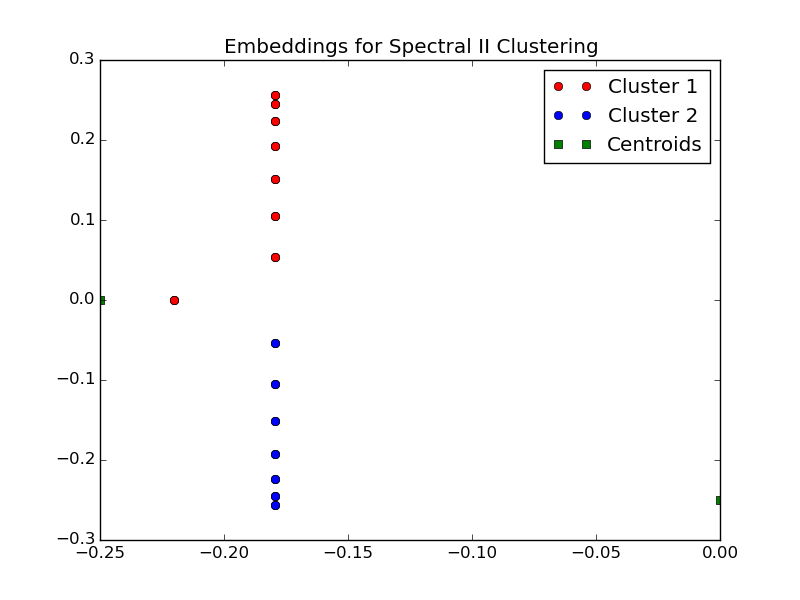
\includegraphics[width=0.5\textwidth]{Embeddings_for_Spectral_II_Clustering.png}

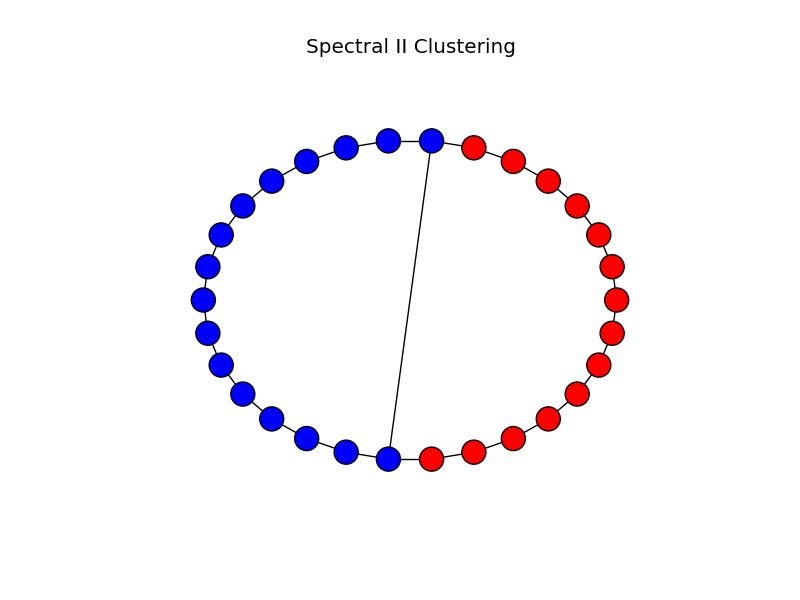
\includegraphics[width=0.5\textwidth]{Spectral_II_Clustering.png}

\end{enumerate}

\end{document}